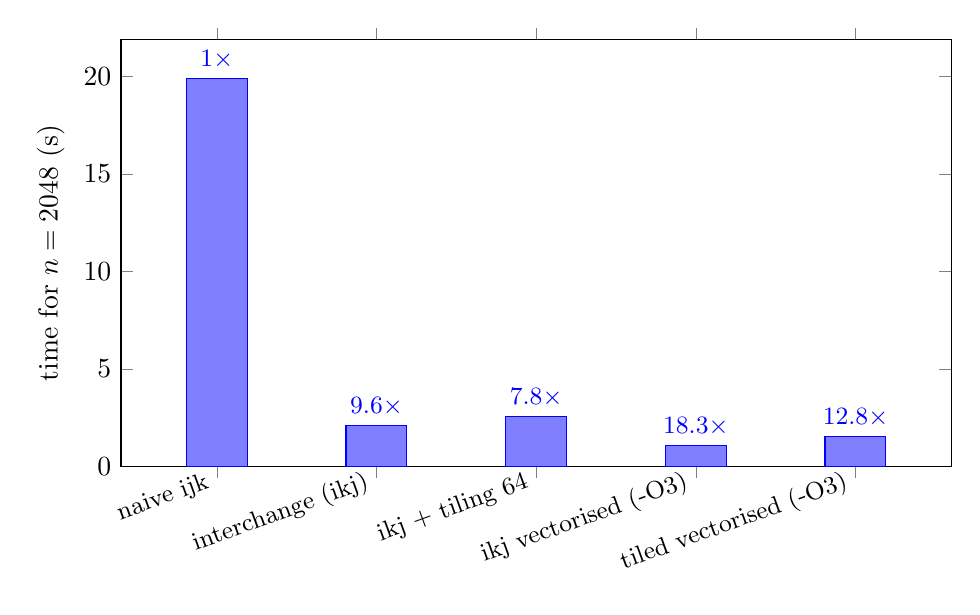
\begin{tikzpicture}
\begin{axis}[ybar, width=\textwidth, height=7cm, bar width=22pt, ymin=0, ylabel={time for $n=2048$ (s)}, symbolic x coords={naive ijk,interchange (ikj),ikj + tiling 64,ikj vectorised (-O3),tiled vectorised (-O3)}, xtick=data,
  x tick label style={rotate=20, anchor=east, font=\small}, nodes near coords={\pgfmathprintnumber[precision=1]{\pgfplotspointmeta}$\times$}, point meta=explicit, nodes near coords style={font=\small}, enlarge x limits=0.15]
\addplot+[fill=blue!50] coordinates {(naive ijk,19.899) [1.0] (interchange (ikj),2.080) [9.6] (ikj + tiling 64,2.539) [7.8] (ikj vectorised (-O3),1.085) [18.3] (tiled vectorised (-O3),1.551) [12.8]};
\end{axis}
\end{tikzpicture}